\subsubsection{Latent Space Temporal Logical Interpolation}
\label{method23}

\begin{figure}[t]
\centering
\subfloat[Latent space temporal logical interpolation module.]{%
    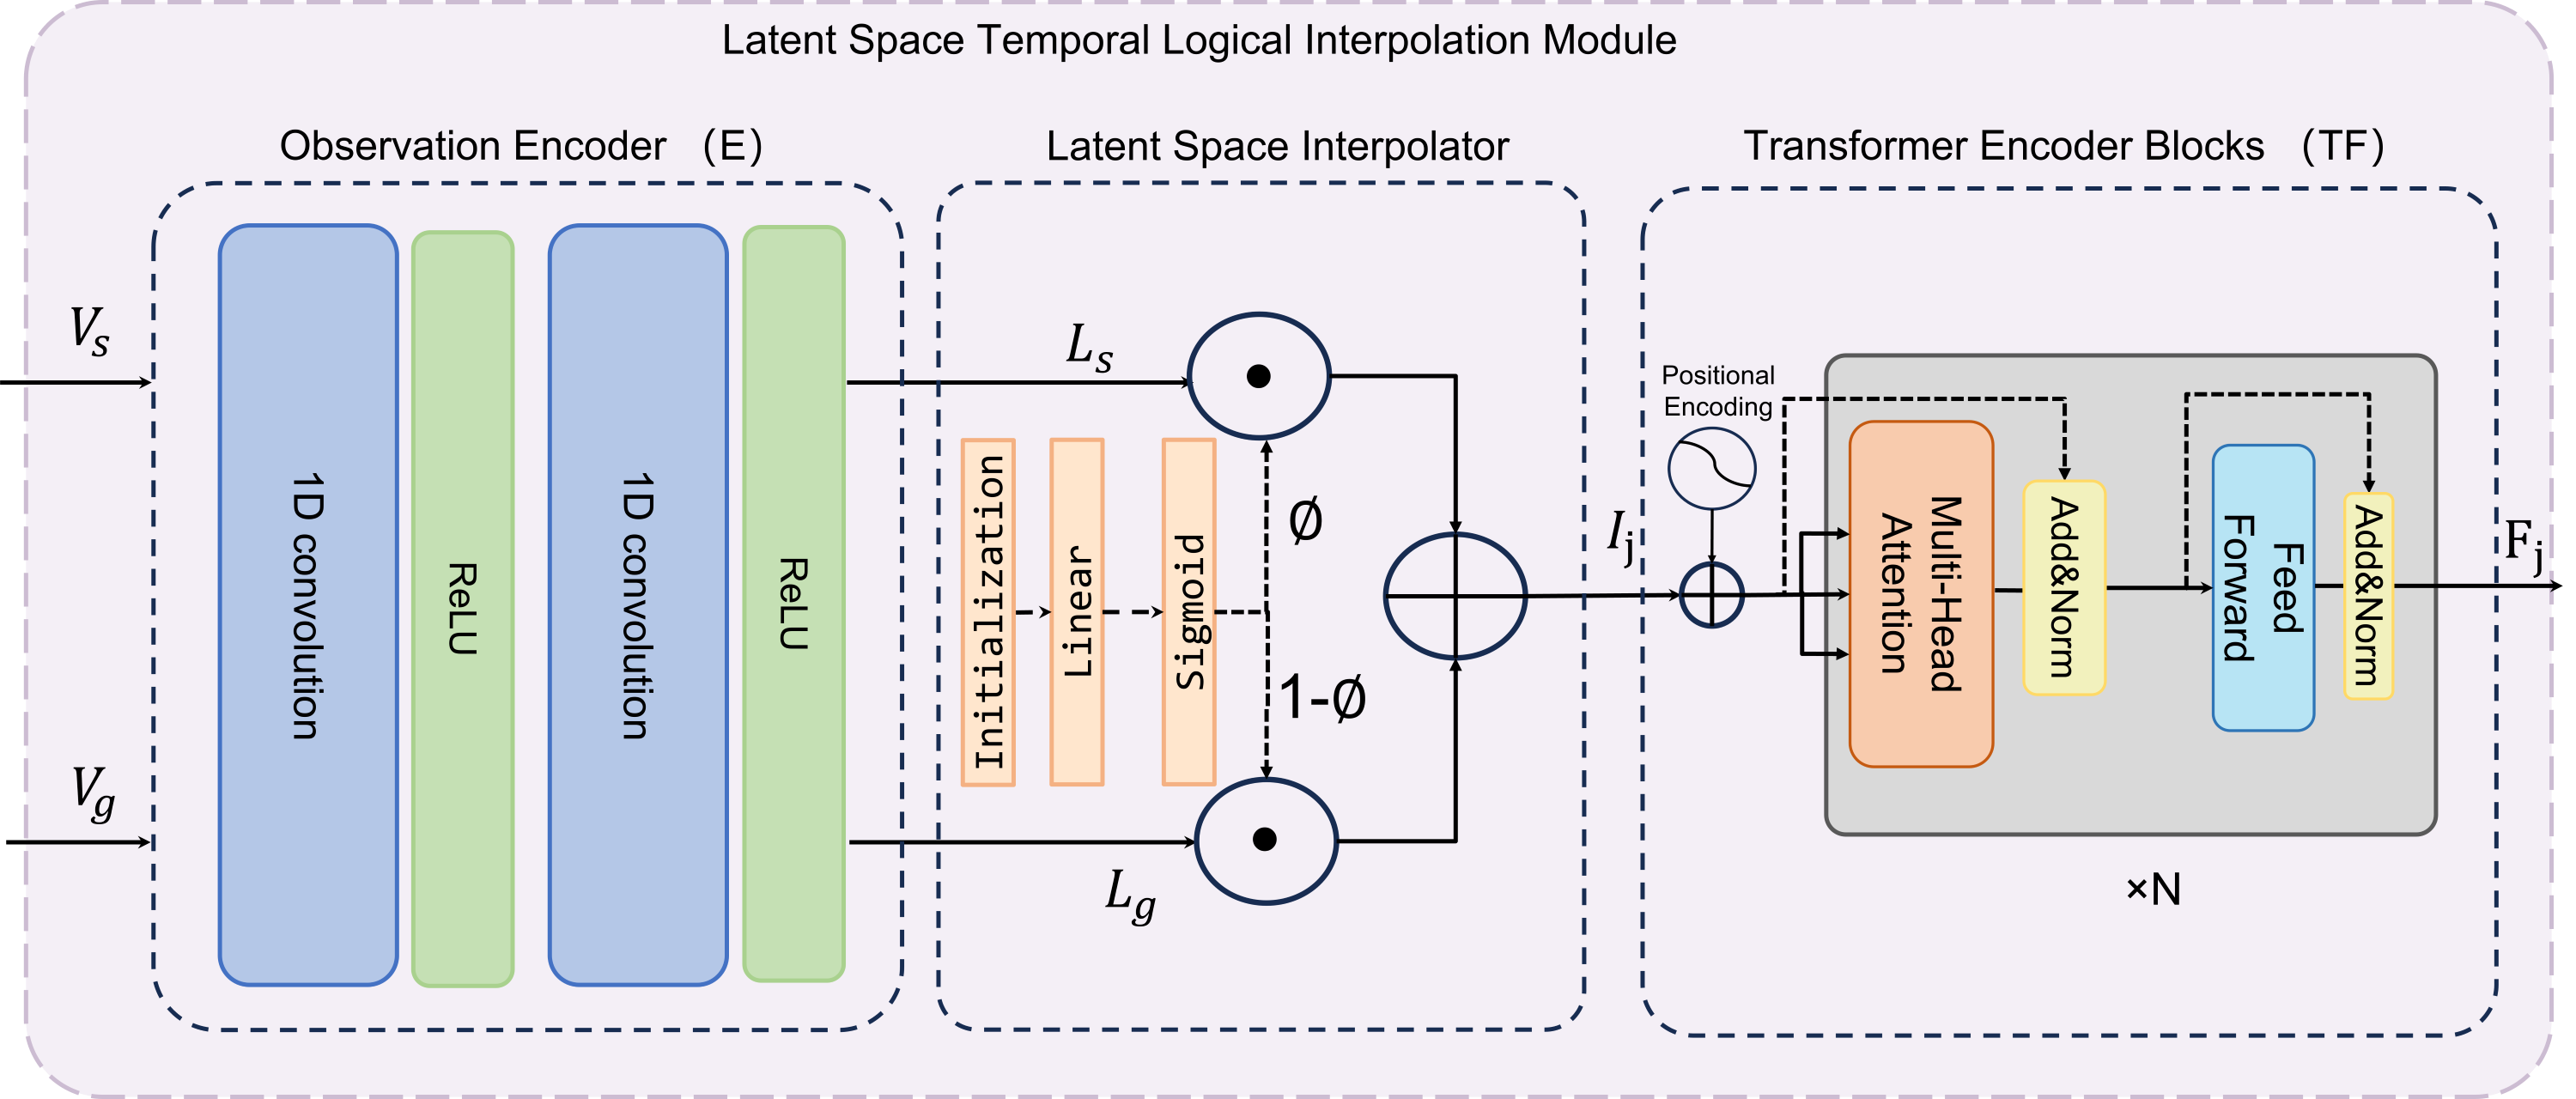
\includegraphics[width=0.48\textwidth, height=0.135\textheight]{figures/architecture2.png}
    \label{fig:architecture2}
}
\hspace{0.1cm} 
\subfloat[Residual temporal block \& cross-attention module.]{%
    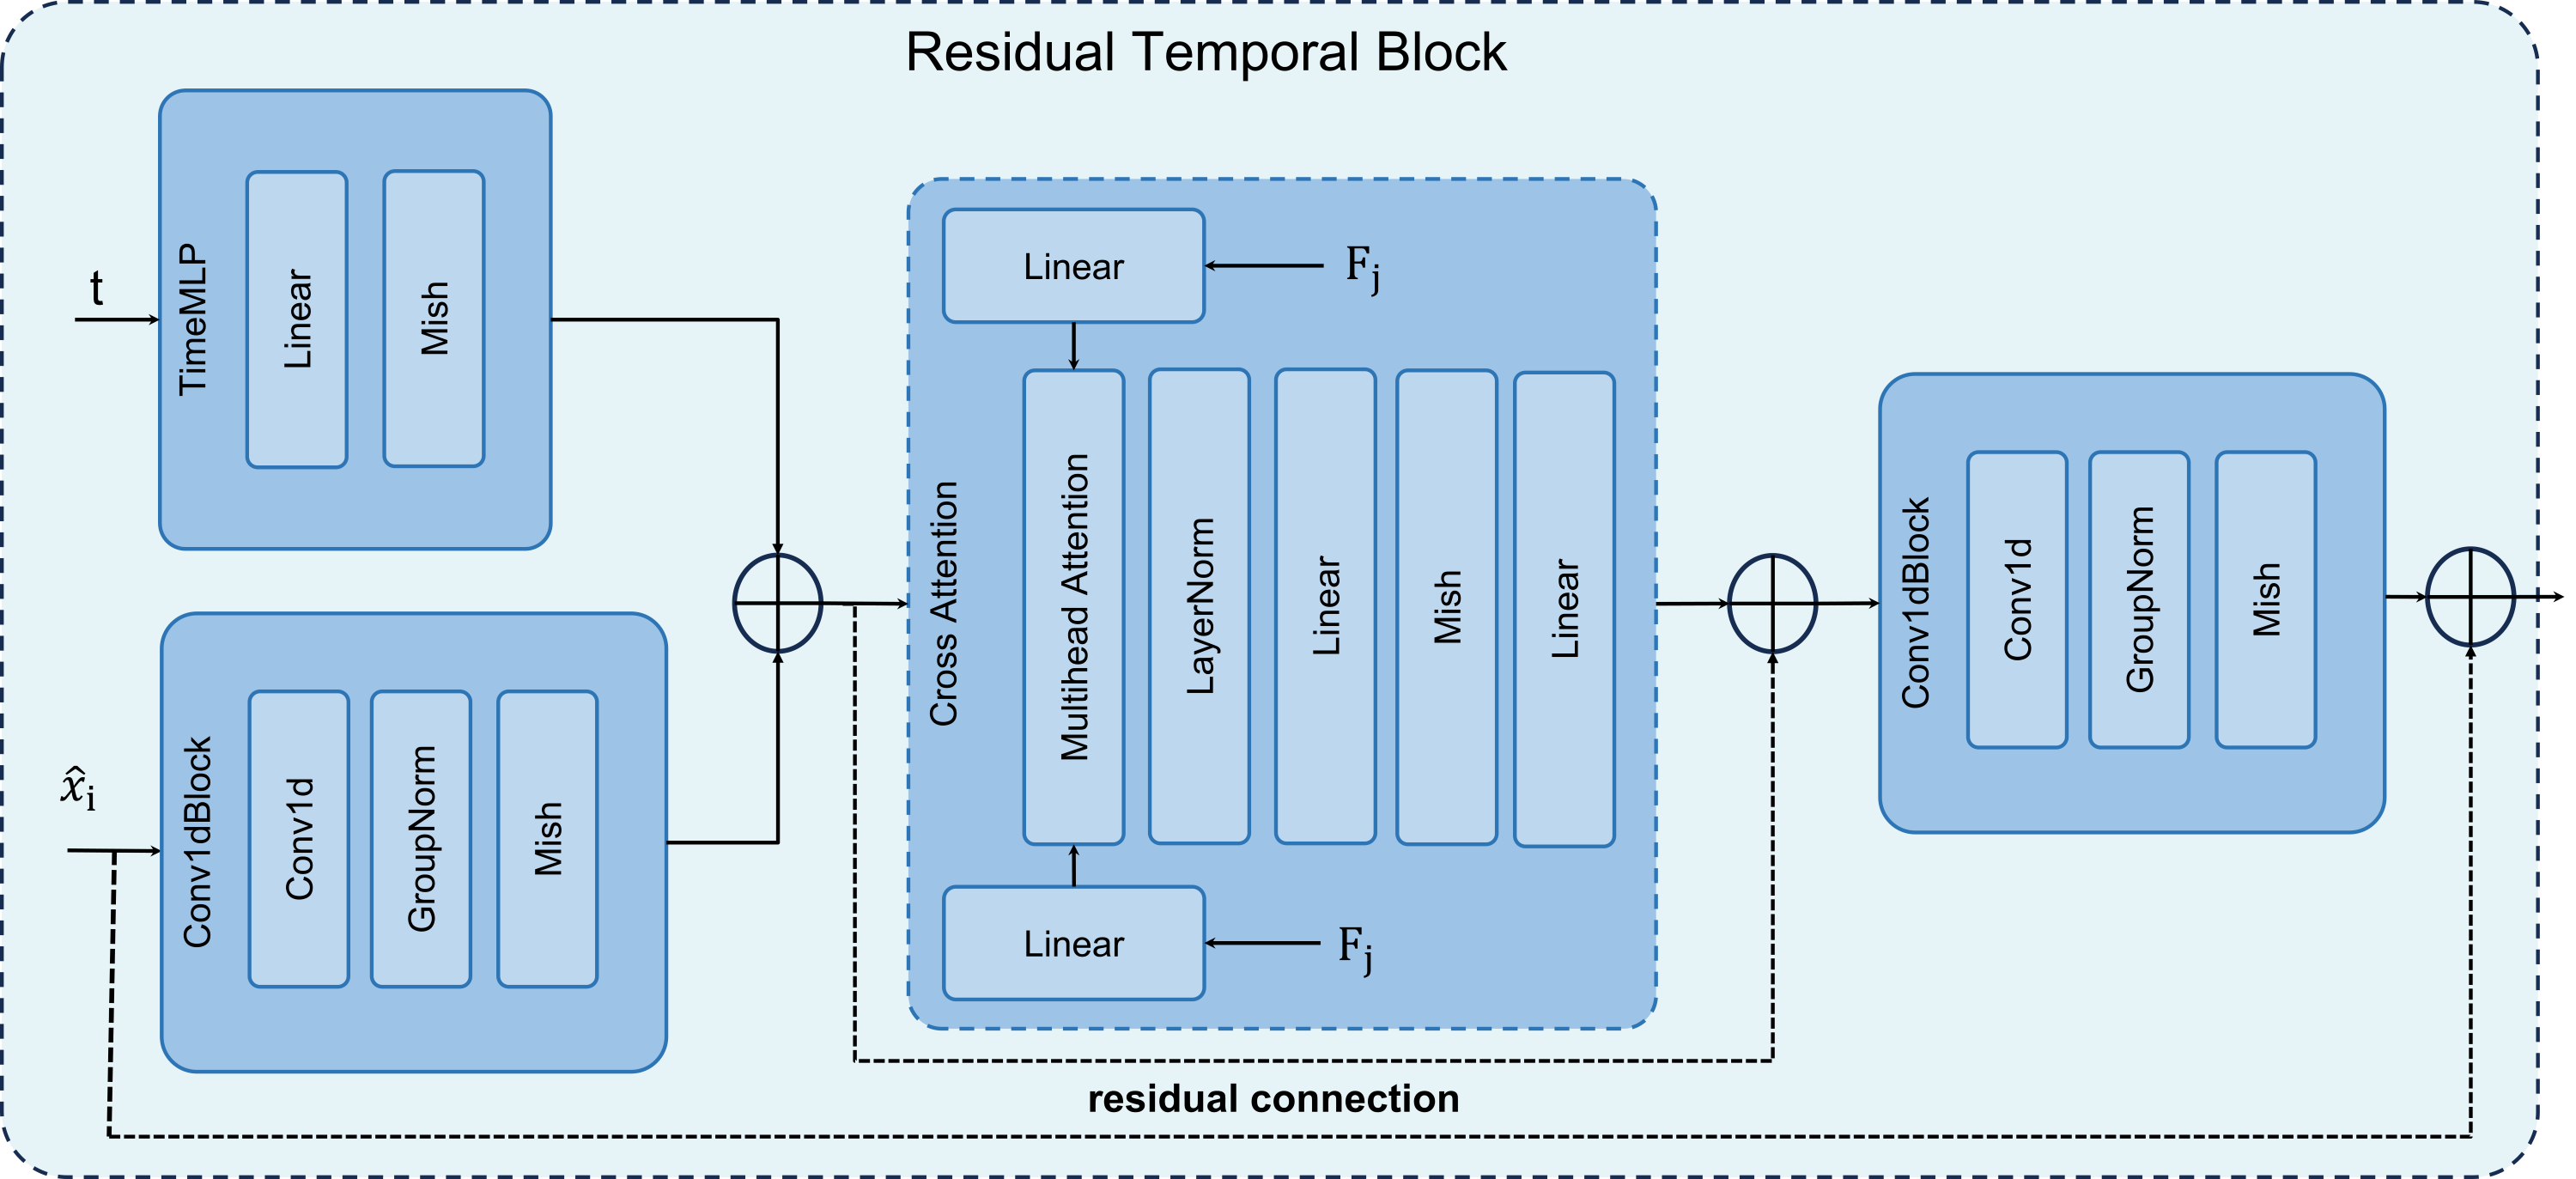
\includegraphics[width=0.48\textwidth, keepaspectratio]{figures/architecture3.png}
    \label{fig:architecture3}
}
\caption{Detailed structure of our interpolation module and cross-attention connection.}
\label{fig:architecturek}
\end{figure}

%and transformer encoder blocks to refine the features and provide more exact information.

As shown in \Cref{fig:architecture2}, the \textbf{Latent Space Temporal Logical Interpolation Module} consists of three core components: an observation encoder, which transforms observation visual features into latent features; a latent space interpolator, which generates multiple features to fill the intermediate supervision; and transformer encoder blocks, which refine the generated features and enhance the module's ability to model the temporal correlations among action sequences.


Specifically, this module first employs an observation encoder $E$, consisting of convolutional layers, to transform the visual observations $V_s$ and $V_g$ into their respective latent features $L_s$ and $L_g$:
\begin{equation}
    L_s, L_g = E(V_s, V_g).
\end{equation}
In the latent space, we perform linear interpolation between $L_s$ and $L_g$ to generate a sequence of interpolated features \{$I_1, I_2, \dots, I_M$\}. 
Unlike fixed linear interpolation, our method dynamically adjusts the interpolation through the learnable interpolation matrix  $\phi \in \mathbb{R}^{M \times O}$ to facilitate smooth and task-specific transitions. 
This matrix, restricted between 0 and 1, is responsible for weighting the latent features $L_s$ and $L_g$ to generate the intermediate latent features as follows:
\begin{equation}
    \begin{split}
        \phi &= Sigmoid(W \cdot \mathbf{\tau} + k), \\
        I_j &= (1 - \phi_j) \cdot L_s + \phi_j \cdot L_g,
    \end{split}
\end{equation}
where $W \in \mathbb{R}^{M \times O}$ and $k \in \mathbb{R}^{M \times O}$ are the parameters of the linear layer, and $O$ represents the observation dimension. The matrix $\mathbf{\tau} \in \mathbb{R}^{M \times O}$ is a learnable matrix initialized with a constant value, controlling a variable ratio between $L_s$ and $L_g$. This method requires no parameter tuning and offers better adaptability to different tasks. The number of latent features $M$ depends on the number of residual temporal blocks in the model.



The sequence of interpolated features $\{I_1, I_2, \dots, I_M\}$ is then passed through a series of transformer encoder blocks $TF$ to obtain the enhanced latent features:
\begin{equation}
    F_1, F_2, \dots, F_M = TF(I_1, I_2, \dots, I_M).
\end{equation}
The self-attention mechanism in the transformers captures dependencies between latent features at different time steps by computing attention scores across all latent features. Stacking multiple transformer blocks allows the model to iteratively refine these features, ensuring that temporal and contextual relationships are effectively learned.


% With these latent features  containing temporal logical information, 

To integrate the interpolated latent features $\{F_1, F_2, \dots, F_M\}$ into the model during the denoising process, we incorporate cross-attention layers~\citep{khachatryan2023text2video} into the residual temporal blocks of the U-Net, as shown in \Cref{fig:architecture3}. This allows the model to dynamically focus on relevant latent features through a learnable matrix, enhancing its ability to capture complex relationships with more latent temporal logical information and improving the quality of action predictions.

In this setup, the latent feature $F_j$, processed through a linear layer, serves as the key and value, while $\hat{x}_n$, processed through a convolutional block and combined with $t$ (sampled from random integers), acts as the query. The cross-attention is computed as:
\begin{equation}
    \hat{x}_n = softmax\left(\frac{\left[CB(\hat{x}_n) + TM(t)\right] \cdot LF_j^T}{\sqrt{O}}\right) \cdot LF_j,
\end{equation}
where $CB$ denotes a 1D convolution block, $TM$ represents a time MLP, and $LF_j$ refers to the result obtained from passing $F_j$ through a linear layer. This design enables the model to effectively capture temporal logical relationships, thereby improving the overall quality of action prediction.

